\section{Badany obiekt}
\label{sec:badany-obiekt}
Rakieta FOK 2 jest wyposażoną w głowicę obrazującą ewolucją rakiety sterowanej FOK.
Rakieta, przedstawiona na~Rysunku~\ref{fig:badany-obiekt-fok}, sterowana jest aerodynamicznie za pomocą 4~sterów umieszczonych przed
środkiem masy (canardów). Napędzana jest silnikiem na stały materiał pędny o impulsie około
\SI{1000}{\N\s}. Pozwala to jej osiągnąć pułap \SI{1000}{\m} oraz liczbę Macha \num{0.4}.
Parametry rakiety FOK 2 przedstawiono w Tabeli~\ref{tab:badany-obiekt-parametry-rakiety}.
Wymiary rakiety przedstawiono na Rysunku~\ref{fig:badany-obiekt-fok-szkic}.
Obecnie rozwijany jest nowy zespół napędowy - BEM \cite{michal}. 
Wraz z odchudzeniem reszty rakiety pozwoli on na znaczny wzrost osiągów rakiety - osiągnięcie liczby Macha \num{0.7} i pułapu \SI{3}{\kilo\m}. 
Celem rakiety FOK 2 jest lot do celu z użyciem nawigacji wizyjnej. 
Na dzień stworzenia pracy rakieta ta odbyła 5 testów lotnych podczas których 
zbierane były dane do identyfikacji modelu aerodynamicznego rakiety oraz 
podjęte były próby pionizacji rakiety. Niestety żadna z podjętych misji
pionizacyjnych nie zakończyła się powodzeniem.

\begin{figure}[htbp]
    \centering
        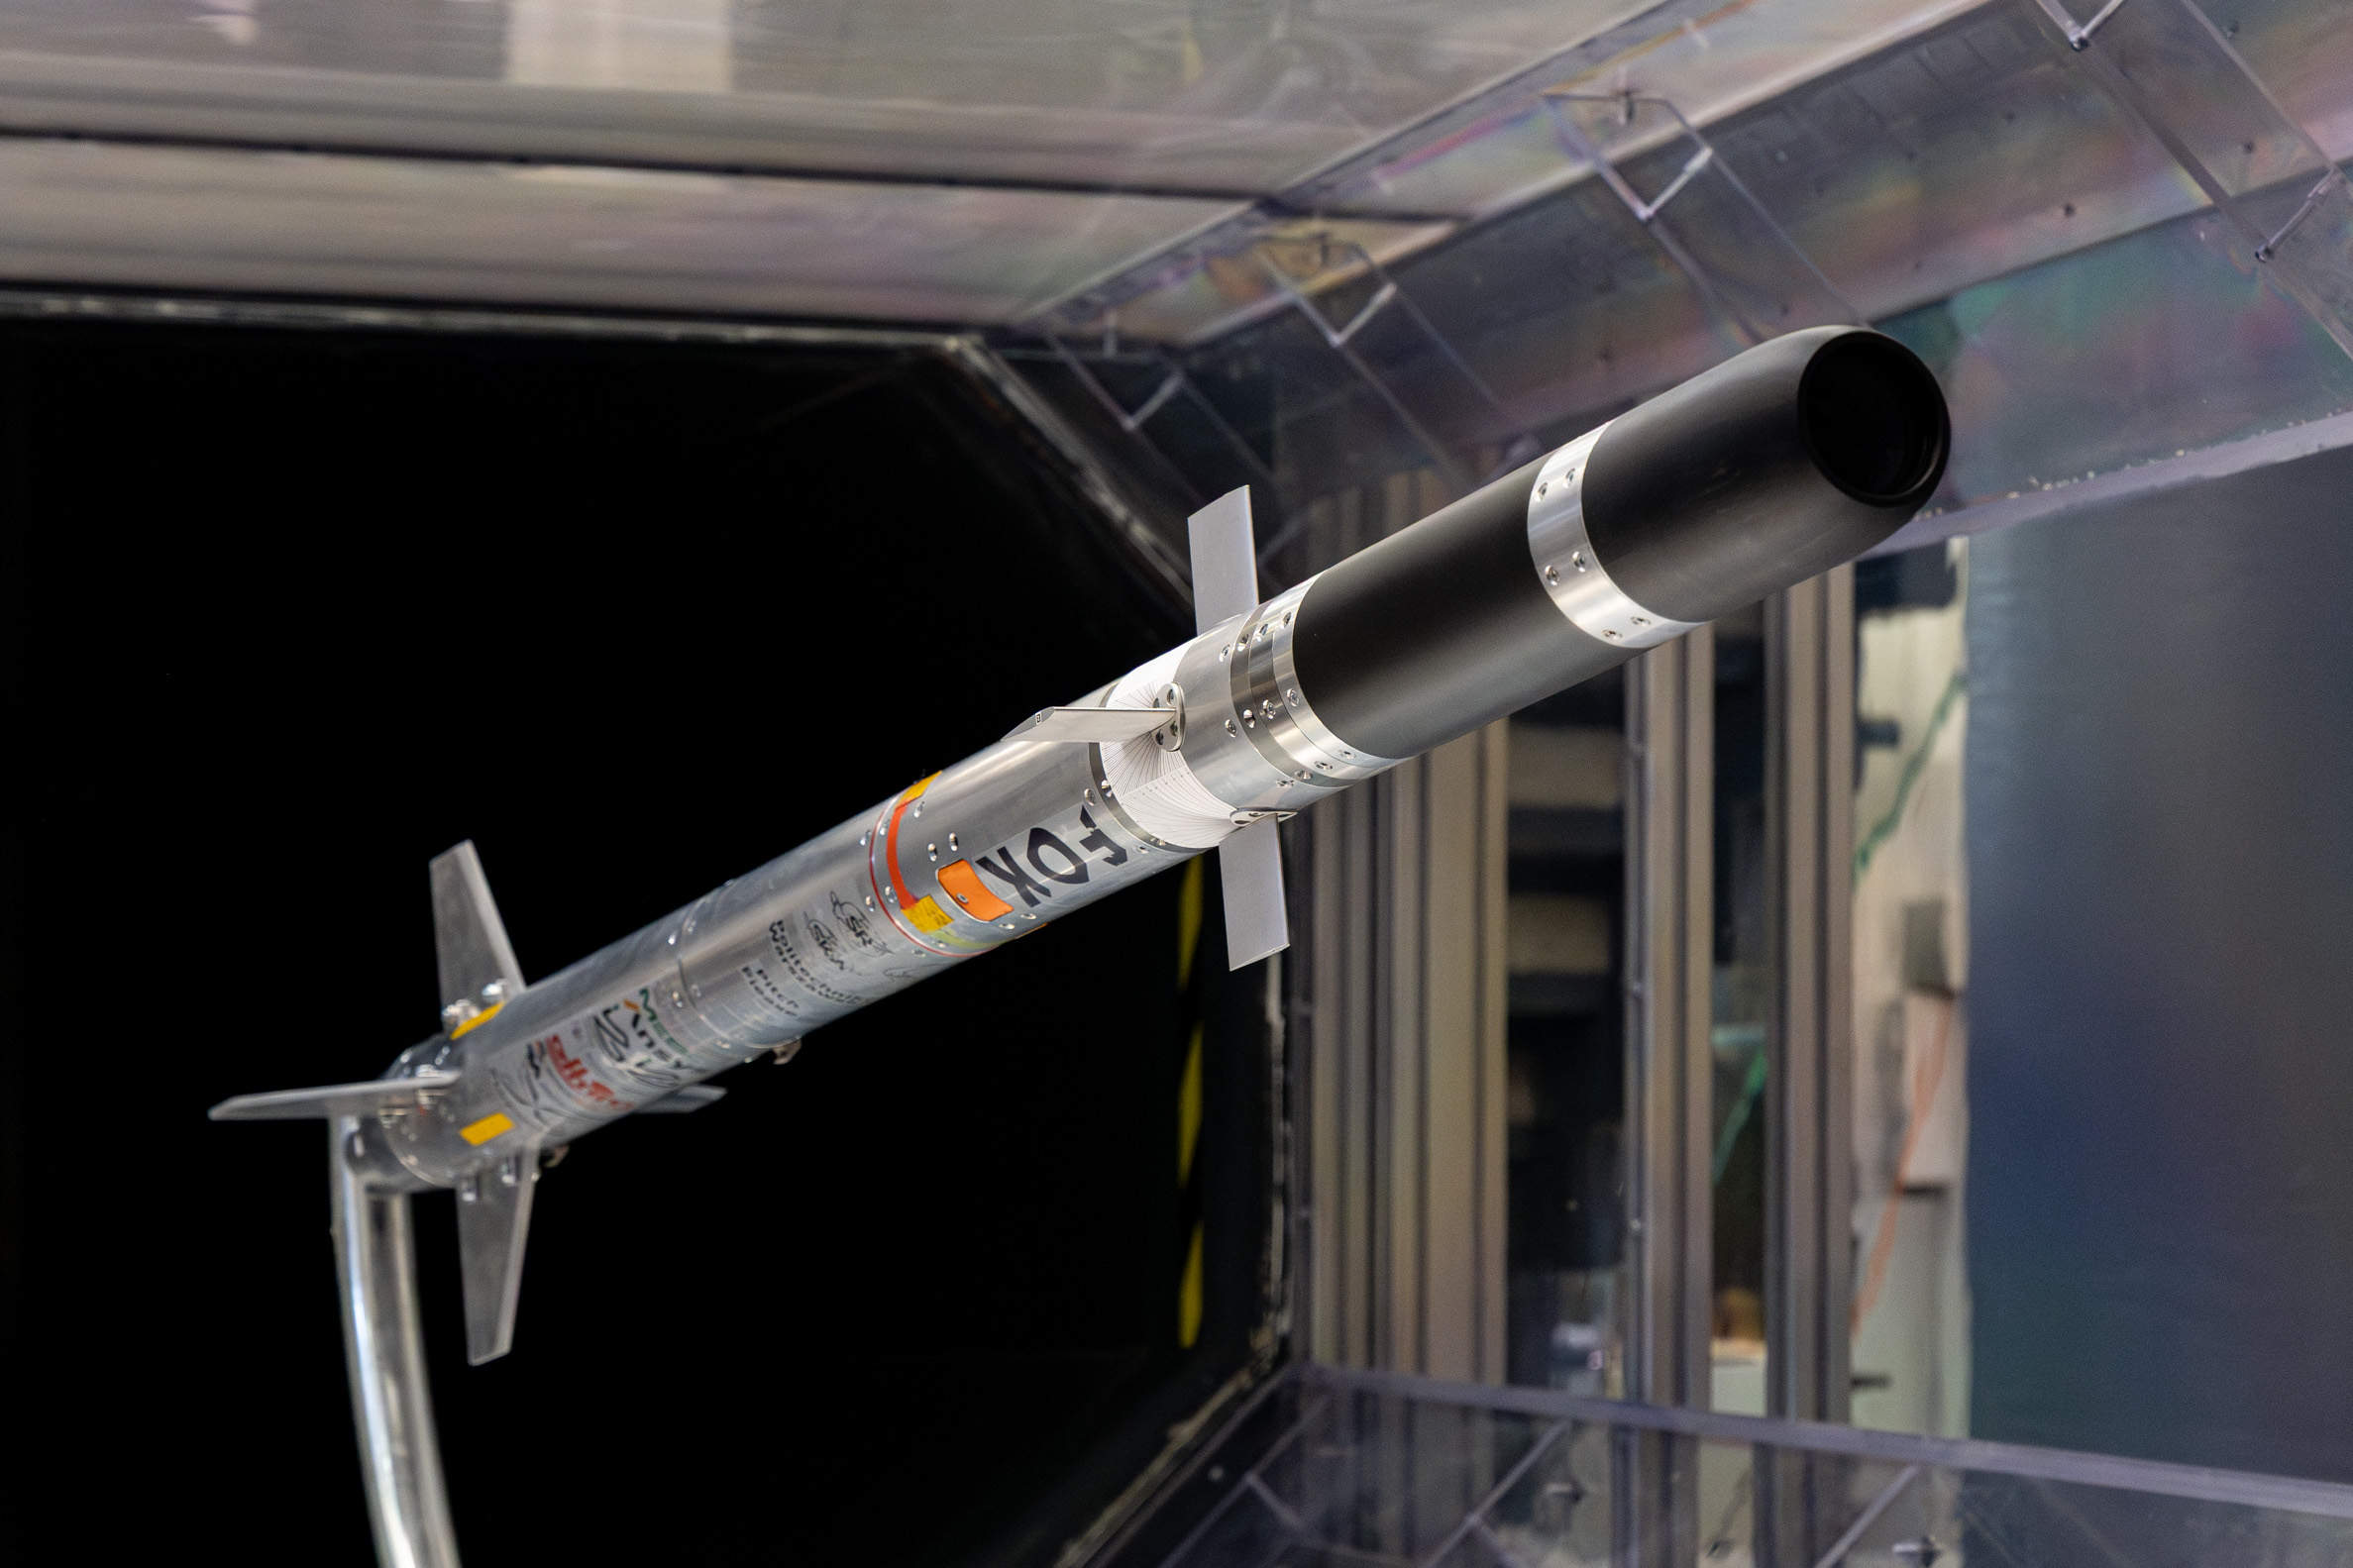
\includegraphics[width=0.8\linewidth]{Figures/fok_tunnel.JPG}
    \caption{Rakieta FOK 2 w tunelu aerodynamicznym}
    \label{fig:badany-obiekt-fok}
\end{figure}

\begin{figure}[htbp]
    \centering
    
\includegraphics[width=0.95\textwidth, trim={18cm, 55cm, 22cm, 5cm},clip]{FOKdraft.pdf}
    \caption{Wymiary rakiety FOK 2}
    \label{fig:badany-obiekt-fok-szkic}
\end{figure}


\begin{table}[htbp]
    \centering
    \caption{Parametry rakiety FOK 2.}
    \label{tab:badany-obiekt-parametry-rakiety}
    \begin{tabular}{lll}
        \toprule
        Parametr & Wartość & Jednostka \\
        \midrule
        Masa startowa & 6,0 & \si{\kg} \\
        Długość & 1,3285 & \si{\m} \\
        Średnica & 0,075 & \si{\m} \\
        Impuls całkowity & 1000 & \si{\N\s} \\
        Masa materiału pędnego & 0,5 & \si{\kg} \\
        Pułap & 1000 & \si{\m} \\
        \bottomrule
    \end{tabular}
\end{table}

\subsection{System sterowania rakiety}
\label{subsec:badany-obiekt-system-sterowania}
Docelowa pętla sterowania (Rysunek~\ref{fig:badany-obiekt-system-sterowania-petla}) rakiety FOK 2 opiera się na interakcji między głowicą optoelektroniczną,
czujnikiem INS/GNSS, komputerem pokładowym i układem wykonawczym systemu sterowania.
W tej pracy rozważane są konfiguracje rakiety bez informacji z głowicy w pętli sterowania.


\begin{figure}[htbp]
    \centering
        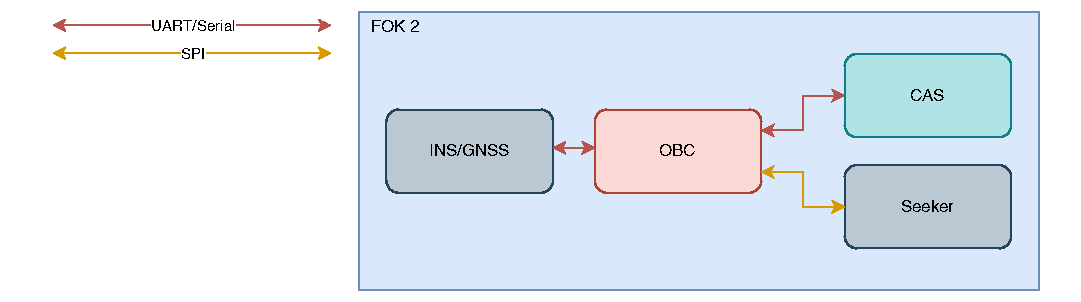
\includegraphics[width=0.8\linewidth]{Figures/foksimplediagram.pdf}
    \caption{Pętla sterowania rakiety FOK 2}
    \label{fig:badany-obiekt-system-sterowania-petla}
\end{figure}

\subsubsection{Komputer pokładowy}
\label{subsubsec:badany-obiekt-system-sterowania-komputer}
Komputer pokładowy rakiety FOK 2 opiera się na Raspberry Pi Pico 2 W.
Został on wybrany przez łatwość pisania oprogramowania na tej platformie.
Oprogramowanie komputera pokładowego jest autorskie, oparte na 
systemie czasu rzeczywistego FreeRTOS \cite{freertos}.
Podczas lotu zbiera on informacje za pomocą protokołu UART z czujnika. 
Także z użyciem tego protokołu komunikuje się z serwomechanizmami. 
Z głowicą komunikuje się za pomocą protokołu SPI, druga
instancja tego protokołu jaką dysponuje Pico jest przeznaczona na obsługę
pamięci flash zapisującej stan misji.
Przewodowe możliwości komunikacji z mikrokontrolerem uzupełnia port USB,
po którym jest udostępniona konsola umożliwiająca konfigurację i komunikację 
z komputerem pokładowym. Ponad wymienione interfejsy jest jeszcze WiFi,
które podczas testu lotnego służy do nadawania telemetrii przez komputer pokładowy gdy rakieta znajduje się na wyrzutni.
Interfejs ten zyskuje na znaczeniu podczas testów HIL przeprowadzanych na komputerze osobistym,
podczas których służy do przekazywania stanu rakiety z symulacji do komputera pokładowego rakiety
i pożądanego wychylenia sterów do symulacji. Podczas testów HIL przeprowadzanych na komputerze czasu rzeczywistego
może służyć do transmisji stanu komputera pokładowego w celu jego zapisu do dalszej analizy.

\subsubsection{Układ wykonawczy systemu sterowania}
\label{subsubsec:badany-obiekt-system-sterowania-uklad-wykonawczy}
Układ wykonawczy badanej w pracy konfiguracji rakiety FOK 2 (FOK 2D) składa się z:
\begin{itemize}
    \item serwomechanizmów HerkuleX DRS 0101,
    \item redukującej przekładni zębatej o przełożeniu $i_\tn{w} = \frac{55}{20} = 2,\!75$,
    \item steru o profilu NACA 0009 i wymiarach przedstawionych na Rysunku~\ref{fig:badany-obiekt-fok-szkic},
    \item elementów struktury mechanicznej i oprzyrządowania elektronicznego.
\end{itemize}

\begin{figure}[H]
    \centering
    
\includegraphics[width=0.8\textwidth]{canard_mechanika.pdf}
    \caption{Układ wykonawczy systemu sterowania rakiety FOK 2}
    \label{fig:badany-obiekt-system-sterowania-uklad-wykonawczy-mechanika}
\end{figure}

W nowszych wersjach rakiety (od FOK 2E) używany jest układ wykonawczy nieoparty o koła zębate, a o popychacze.
Wprowadza to drobne nieliniowości w przełożeniu oraz prowadzi do konieczności ponownego przeprowadzenia części testów identyfikujących 
parametry układu wykonawczego. Zmiana wynikała głównie z chęci eliminacji luzów występujących w systemie sterowania rakiety.

\subsubsection{Jednostka pomiarowa INS/GNSS}
\label{subsubsec:badany-obiekt-system-sterowania-czujnik}
W rakiecie używana jest jednostka pomiarowa INS/GNSS VectorNav 200 \cite{vectornav_vn200}. 
% \todo[inline]{Napisać więcej o vnavie}
Pozwala ona na wyznaczenie parametrów lotu rakiety. Komunikacja między rakietą a czujnikiem odbywa się za pomocą protokołu UART.
Został stworzony i umieszczony w symulacji HIL symulator pakietów czujnika, który pozwala na bezpośrednie wpięcie symulacji w pętle sterowania rakiety.
Model czujnika używany w symulacji jest minimalny, pozbawiony symulacji niepewności i szumów. Planowane jest zaimplementowanie 
dokładniejszego modelu czujnika, który pozwoli na weryfikację działania algorytmu sterowania rakiety w warunkach bardziej zbliżonych do rzeczywistych.

